\documentclass[border=0.125cm]{standalone}
\usepackage{tikz}
\usetikzlibrary{positioning}
\usepackage{ifthen}
\usetikzlibrary{matrix,arrows.meta,quotes,shadows,decorations.pathreplacing,positioning,fadings}
\usepackage{cfr-lm}
\usetikzlibrary{shapes.misc}

\begin{document}
	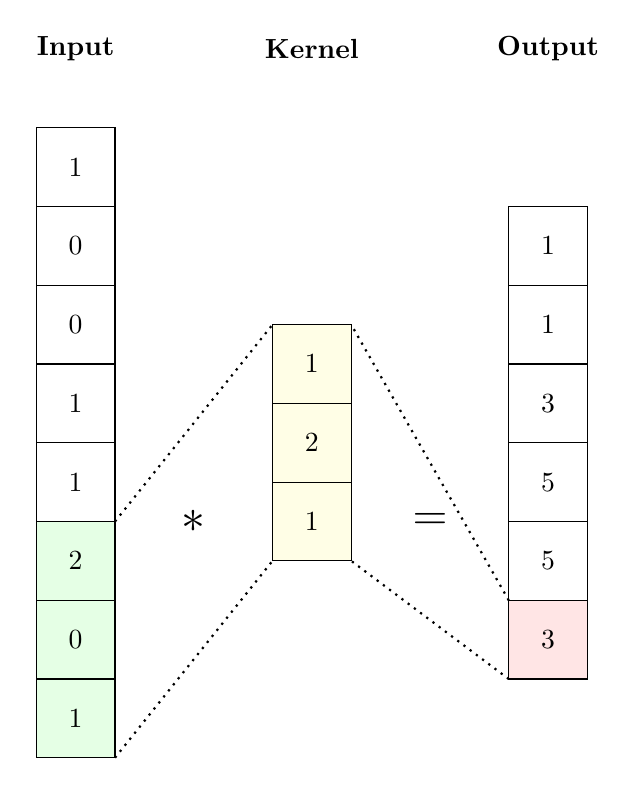
\begin{tikzpicture}
	
		\draw[dotted, thick] (1,4) -- (3,6.5);  
		\draw[dotted, thick] (1,1) -- (3,3.5);  
		
		\draw[dotted, thick] (6,3) -- (4,6.5);  
		\draw[dotted, thick] (6,2) -- (4,3.5);  
		
		\node () at (0.5,10) {\textbf{Input}};
		\node () at (3.5,10) {\textbf{Kernel}};
		\node () at (6.5,10) {\textbf{Output}};
		
		\node () at (2, 4) {\LARGE$\mathbf{*}$};
		\node () at (5, 4) {\LARGE$\mathbf{=}$};
		
		\draw[fill=green!10] (0,1) rectangle (1,4);
		
		\foreach \m/\l [count=\y] in {1,0,2,1,1,0,0,1}
		{
			\draw (0,\y) rectangle  (1,1+\y);
			\node (input-\m) at (0.5, 0.5+\y) {\m};
		}
			
		\draw[fill=yellow!10] (3,3.5) rectangle (4,6.5);
	
		\foreach \m/\l [count=\y] in {1,2,1}
		{
			\draw (3,2.5+\y) rectangle  (4,3.5+\y);
			\node (input-\m) at (3.5, 3+\y) {\m};
		}	
	
		\draw[fill=red!10] (6,2) rectangle (7,3); 	
	
		\foreach \m/\l [count=\y] in {3,5,5,3,1,1}
		{
			\draw (6,1+\y) rectangle  (7,2+\y);
			\ifthenelse{
				\equal{\m}{miss}
			}{
			}
			{
				\node (output-\m) at (6.5, 1.5+\y) {\m}; 
			}
		}
	

	
	
	\end{tikzpicture}
\end{document}